\chapter{Lampiran Pengujian Eksperimental}
\label{lamp:B}

\section{Kuesioner}
\label{sec:survey}
Kuesioner diawali dengan pertanyaan :
\begin{figure}[H]
	\centering  
	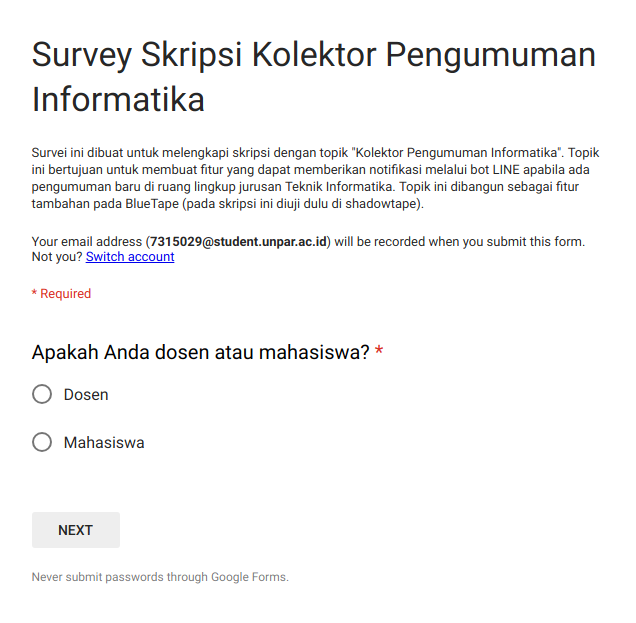
\includegraphics[scale=0.5]{./Survey-Kuesioner/Q0.png}  
	\caption[Kuesioner bagian pertama]{Kuesioner bagian pertama} 
	\label{fig:q0} 
\end{figure}

Apabila responden memilih "Dosen", maka responden akan dialihkan ke bagian Dosen (Lampiran \ref{subsec:survey-dosen}). Apabila responden memilih "Mahasiswa", maka responden akan dialihkan ke bagian Mahasiswa (Lampiran \ref{subsec:survey-mahasiswa}). Responden wajib mengisi semua pertanyaan di kuesioner ini kecuali pertanyaan saran.

\subsection{Dosen}
\label{subsec:survey-dosen}
\begin{figure}[H]
	\centering  
	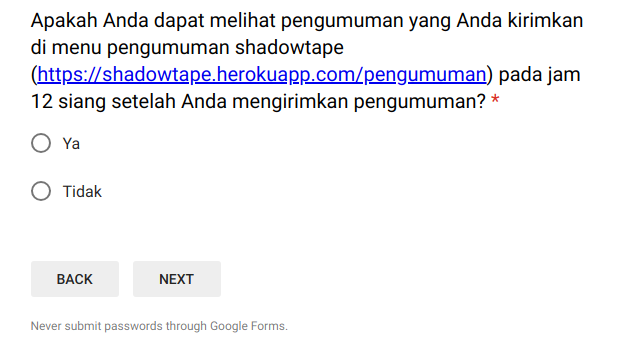
\includegraphics[scale=0.5]{./Survey-Kuesioner/Q1-D1.png}  
	\caption[Kuesioner bagian Dosen pertanyaan pertama]{Kuesioner bagian Dosen pertanyaan pertama} 
	\label{fig:q1-d1} 
\end{figure}

Apabila responden memilih jawaban "Ya" pada pertanyaan pertama (Gambar~\ref{fig:q1-d1}), maka responden akan dialihkan ke pertanyaan kedua (Gambar~\ref{fig:q1-d2}). Apabila responden memilih jawaban "Tidak", maka responden akan dialihkan ke bagian \textit{System Usability Scale} dan Saran (Lampiran \ref{subsec:final}) dan Saran (Gambar~\ref{subsec:final}). 

\begin{figure}[H]
	\centering  
	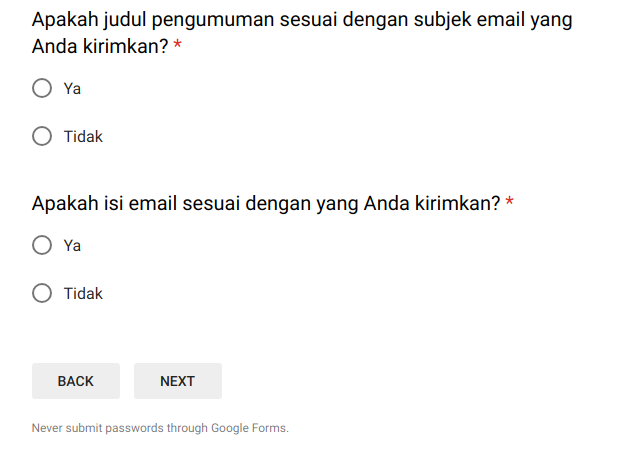
\includegraphics[scale=0.5]{./Survey-Kuesioner/Q1-D2.png}  
	\caption[Kuesioner bagian Dosen pertanyaan kedua dan ketiga]{Kuesioner bagian Dosen pertanyaan kedua dan ketiga} 
	\label{fig:q1-d2} 
\end{figure}

Apabila responden memilih jawaban "Ya" pada pertanyaan ketiga (pertanyaan kedua di Gambar~\ref{fig:q1-d1}), maka responden akan dialihkan ke pertanyaan keempat (Gambar~\ref{fig:q1-d3}). Apabila responden memilih jawaban "Tidak", maka responden akan dialihkan ke bagian \textit{System Usability Scale} dan Saran (Gambar~\ref{subsec:final}). 

\begin{figure}[H]
	\centering  
	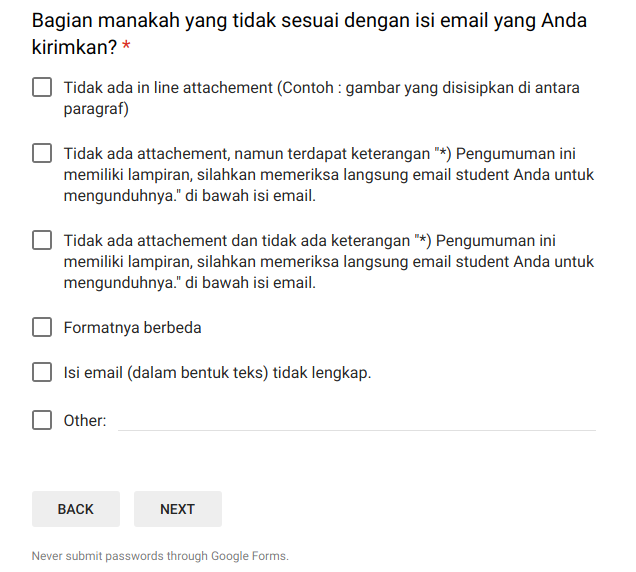
\includegraphics[scale=0.5]{./Survey-Kuesioner/Q1-D3.png}  
	\caption[Kuesioner bagian Dosen pertanyaan keempat]{Kuesioner bagian Dosen pertanyaan keempat} 
	\label{fig:q1-d3} 
\end{figure}

Apapun jawaban responden pada pertanyaan keempat (Gambar~\ref{fig:q1-d3}), responden akan dialihkan ke bagian \textit{System Usability Scale} dan Saran (Gambar~\ref{subsec:final}).

\subsection{Mahasiswa}
\label{subsec:survey-mahasiswa}
\begin{figure}[H]
	\centering  
	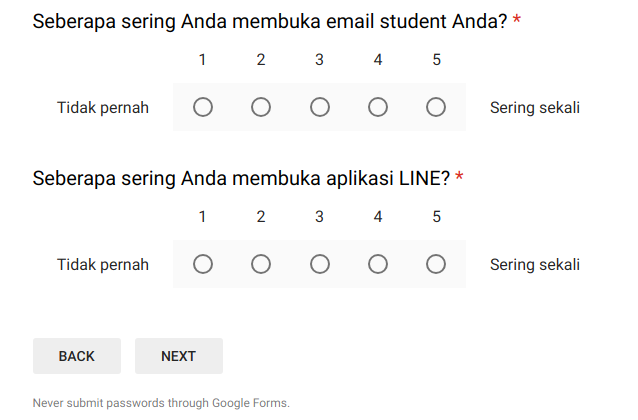
\includegraphics[scale=0.5]{./Survey-Kuesioner/Q1-M1.png}  
	\caption[Kuesioner bagian Mahasiswa pertanyaan pertama dan kedua]{Kuesioner bagian Mahasiswa pertanyaan pertama dan kedua} 
	\label{fig:q1-m1} 
\end{figure}

Apapun jawaban responden pada pertanyaan pertama dan kedua(Gambar~\ref{fig:q1-m1}), responden akan dialihkan ke pertanyaan kedua (Gambar~\ref{fig:q1-m2}).

\begin{figure}[H]
	\centering  
	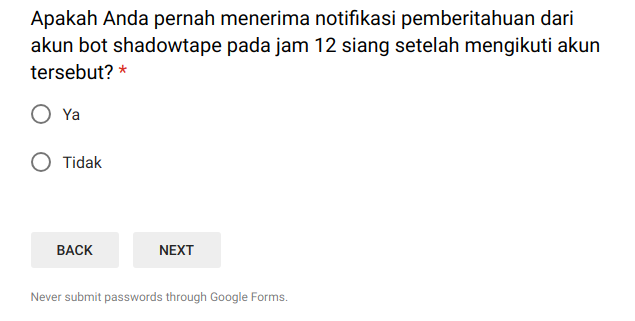
\includegraphics[scale=0.5]{./Survey-Kuesioner/Q1-M2.png}  
	\caption[Kuesioner bagian Mahasiswa pertanyaan ketiga]{Kuesioner bagian Mahasiswa pertanyaan ketiga} 
	\label{fig:q1-m2} 
\end{figure}

Apabila responden memilih jawaban "Ya" pada pertanyaan ketiga (Gambar~\ref{fig:q1-m2}), maka responden akan dialihkan ke pertanyaan keempat (Gambar~\ref{fig:q1-m3}). Apabila responden memilih jawaban "Tidak", maka jawaban responden akan dikirim kepada peneliti.

\begin{figure}[H]
	\centering  
	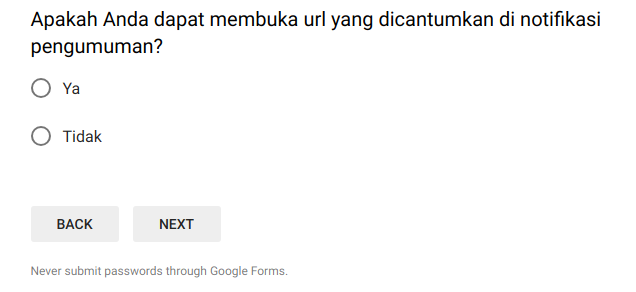
\includegraphics[scale=0.5]{./Survey-Kuesioner/Q1-M3.png}  
	\caption[Kuesioner bagian Mahasiswa pertanyaan keempat]{Kuesioner bagian Mahasiswa pertanyaan keempat} 
	\label{fig:q1-m3} 
\end{figure}

Apabila responden memilih jawaban "Ya" pada pertanyaan keempat (Gambar~\ref{fig:q1-m3}), maka responden akan dialihkan ke pertanyaan kelima (Gambar~\ref{fig:q1-m4}). Apabila responden memilih jawaban "Tidak", maka responden akan dialihkan ke bagian \textit{System Usability Scale} dan Saran (Gambar~\ref{subsec:final}).

\begin{figure}[H]
	\centering  
	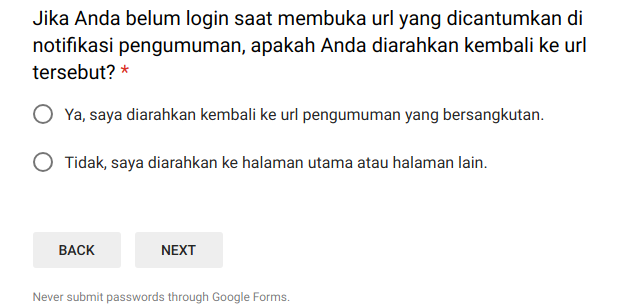
\includegraphics[scale=0.5]{./Survey-Kuesioner/Q1-M4.png}  
	\caption[Kuesioner bagian Mahasiswa pertanyaan kelima]{Kuesioner bagian Mahasiswa pertanyaan kelima} 
	\label{fig:q1-m4} 
\end{figure}

Apapun jawaban responden pada pertanyaan kelima (Gambar~\ref{fig:q1-m4}), responden akan dialihkan ke bagian \textit{System Usability Scale} dan Saran (Gambar~\ref{subsec:final}).

\subsection{\textit{System Usability Scale} dan Saran}
\label{subsec:final}

Bagian ini adalah bagian terakhir dari kuesioner. Bagian ini memiliki 11 pertanyaan yang terdiri dari 10 pertanyaan hasil adaptasi pertanyaan yang ditanyakan saat uji usabilitas dengan metode \textit{System Usability Scale} dan 1 pertanyaan saran. Setelah responden menjawab bagian ini, jawaban responden akan dikirim kepada peneliti. Pertanyaan pada bagian ini ditampilkan pada Gambar~\ref{fig:lq1}, Gambar~\ref{fig:lq2}, dan Gambar~\ref{fig:lq3}.

\begin{figure}[H]
	\centering  
	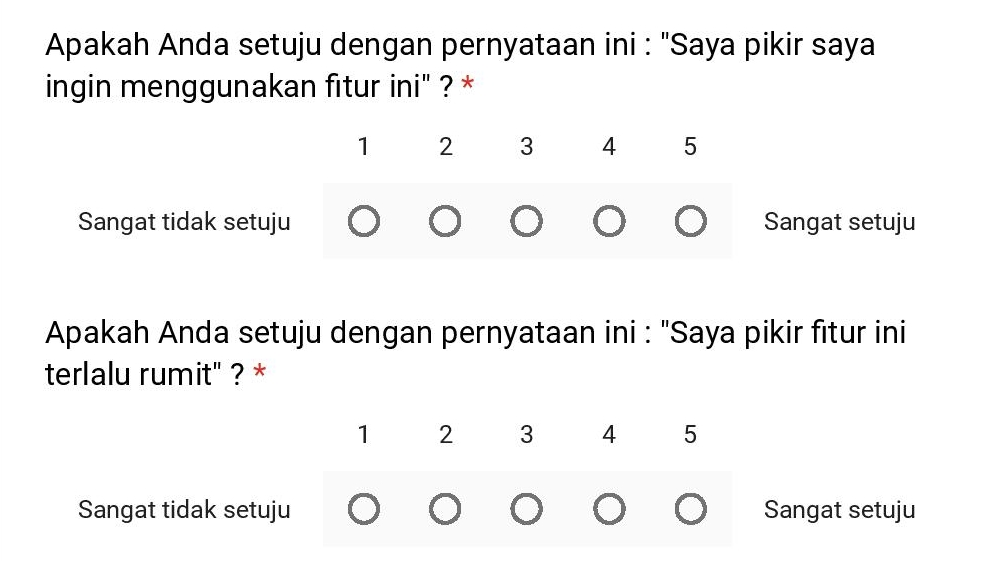
\includegraphics[scale=0.32]{./Survey-Kuesioner/LQ1.jpg} 
	\caption[Kuesioner bagian \textit{System Usability Scale} dan Saran bagian 1]{Kuesioner bagian \textit{System Usability Scale} dan Saran bagian 1} 
	\label{fig:lq1} 
\end{figure}

\begin{figure}[H]
	\centering  
	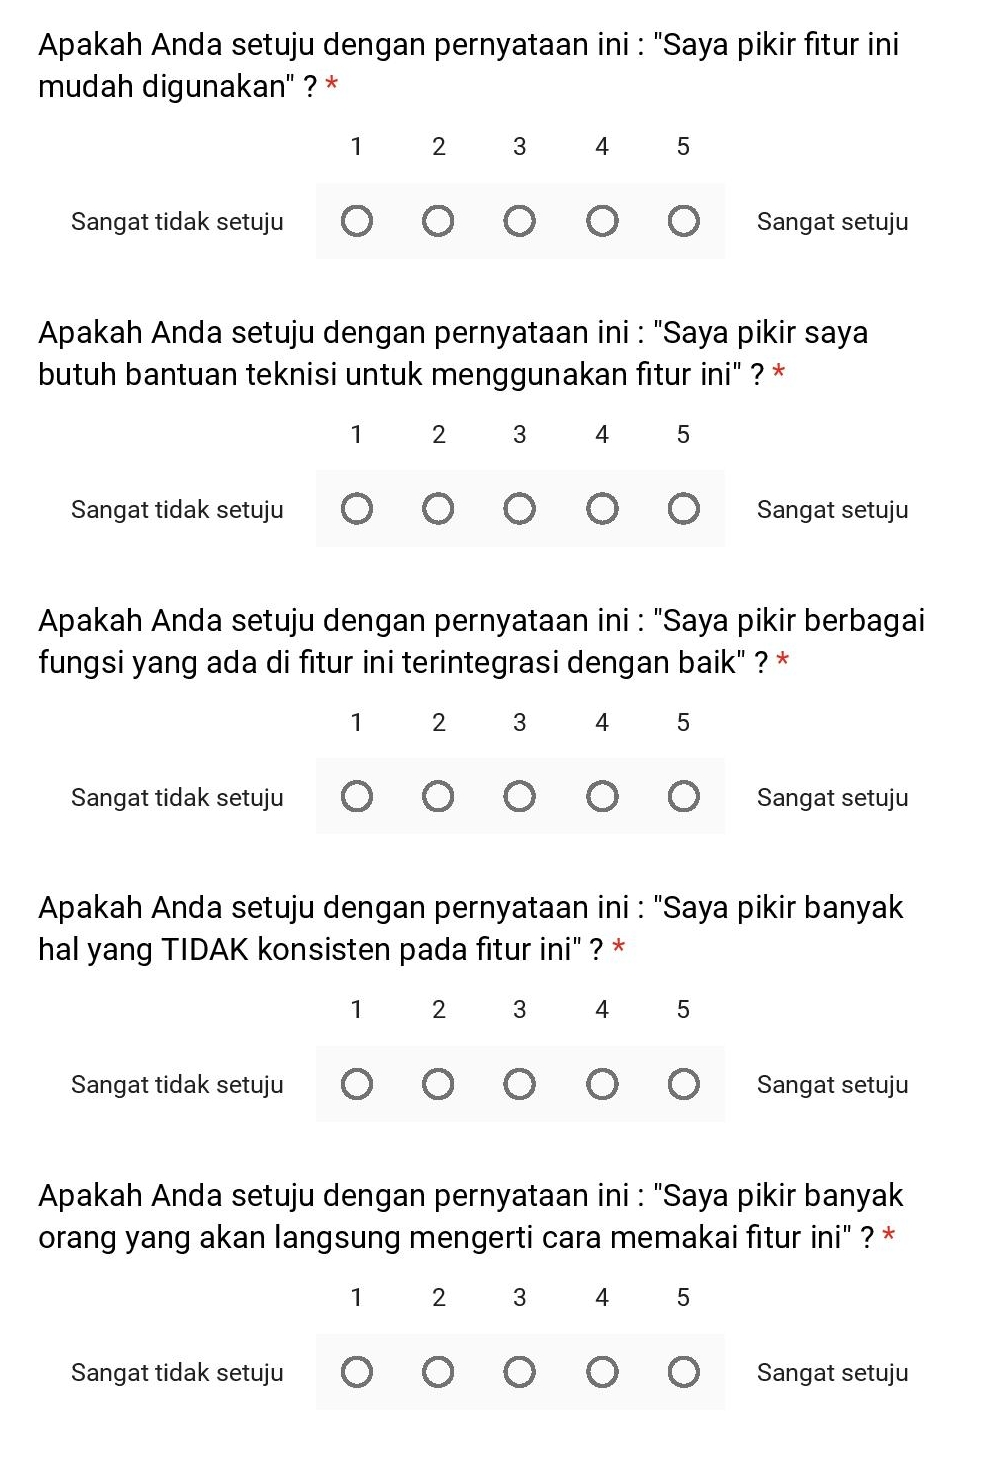
\includegraphics[scale=0.32]{./Survey-Kuesioner/LQ2.jpg}  
	\caption[Kuesioner bagian \textit{System Usability Scale} dan Saran bagian 2]{Kuesioner bagian \textit{System Usability Scale} dan Saran bagian 2} 
	\label{fig:lq2} 
\end{figure}

\begin{figure}[H]
	\centering  
	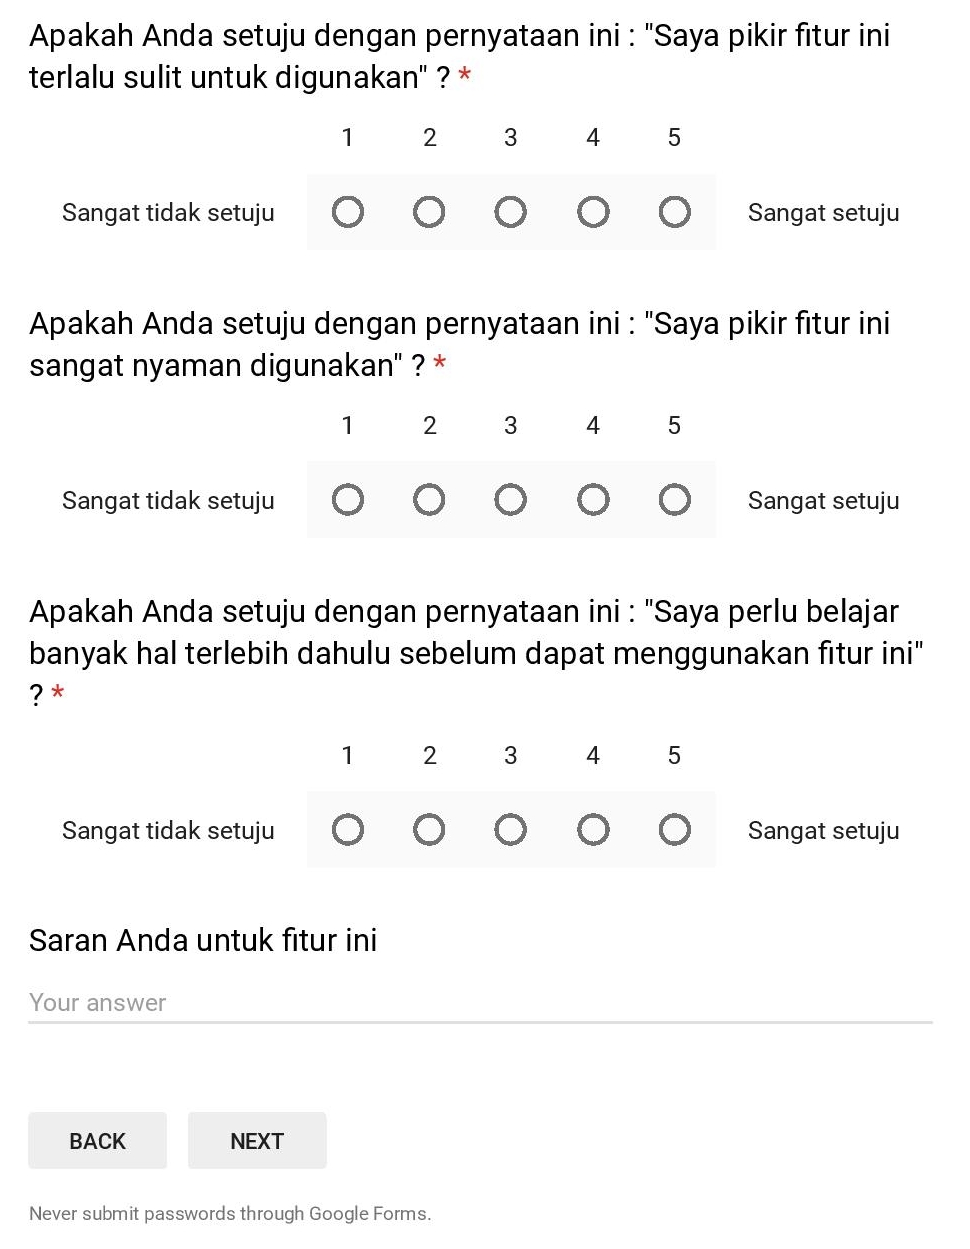
\includegraphics[scale=0.32]{./Survey-Kuesioner/LQ3.jpg}  
	\caption[Kuesioner bagian \textit{System Usability Scale} dan Saran bagian 3]{Kuesioner bagian \textit{System Usability Scale} dan Saran bagian 3} 
	\label{fig:lq3} 
\end{figure}

\label{sec:full-result-survey}
\section{Hasil Mentah Kuesioner}
\begin{table}[H]
	\caption{Hasil Kuesioner Dosen}
	\label{table:hasil-kuesioner-dosen}
	\centering
	\begin{tabular}{|c|c|c|c|c|}
 			\hline
			\textbf{Kode Responden} & \textbf{(1)} & \textbf{(2)} & \textbf{(3)}  & \textbf{(4)} \\
			\hline
			b44980e1427379eb5135f9cf525caff7 & Tidak & - & - & - \\
			\hline
			8759eb252d89ea97ae317b501d29e440 & Ya & Ya & Ya & - \\
            \hline
	\end{tabular}
\end{table}
Keterangan:
\begin{itemize}
\item (1): Apakah Anda dapat melihat pengumuman yang Anda kirimkan di menu pengumuman shadowtape (https://shadowtape.herokuapp.com/pengumuman) pada jam 12 siang setelah Anda mengirimkan pengumuman?
\item (2): Apakah judul pengumuman sesuai dengan subjek \textit{email} yang Anda kirimkan?
\item (3): Apakah isi \textit{email} sesuai dengan yang Anda kirimkan?
\item (4): Bagian manakah yang tidak sesuai dengan isi \textit{email} yang Anda kirimkan?
\end{itemize}

\begin{longtable}{|c|c|c|c|c|c|}
	\caption{Hasil Kuesioner Mahasiswa} 
	\label{table:hasil-kuesioner-mahasiswa} \\
\hline
\textbf{Kode Responden} & \textbf{(1)} & \textbf{(2)} & \textbf{(3)}  & \textbf{(4)} & \textbf{(5)} \\
\hline	baa288c55dbe3374ae2024770ad7d71d	&	3	&	5	&	Ya	&	Tidak	&	-	\\
\hline	30739dd65894243b2fde4fc2c60d7044	&	4	&	5	&	Tidak	&	-	&	-	\\
\hline	da73fa4480f165dc734f00e9e751ed65	&	4	&	4	&	Tidak	&	-	&	-	\\
\hline	6944991200f703e588f514c3132dfb00	&	3	&	5	&	Tidak	&	-	&	-	\\
\hline	c303f0daa68202fece8598e871c3eb2e	&	3	&	5	&	Tidak	&	-	&	-	\\
\hline	87cdf6dccc6c35b09177ee04d9aaba8b	&	3	&	5	&	Tidak	&	-	&	-	\\
\hline	890e85f2f19d33ae01904530aeee6820	&	5	&	5	&	Ya	&	Ya	&	Tidak	\\
\hline	65ba791471cd92bf34cca127c3ea403a	&	4	&	5	&	Tidak	&	-	&	-	\\
\hline	df46a7bc42efcc041f92e505359436ce	&	5	&	5	&	Tidak	&	-	&	-	\\
\hline	5925f011062006b32ac89122779174ca	&	2	&	4	&	Tidak	&	-	&	-	\\
\hline	bd86d293b094f35a23df03ac2827f075	&	2	&	4	&	Tidak	&	-	&	-	\\
\hline	7d9892b660298864ec00bbef71558b31	&	4	&	5	&	Ya	&	Tidak	&	-	\\
\hline	f5571c6dbcc9b28db2c83d478a78a9c9	&	5	&	5	&	Tidak	&	-	&	-	\\
\hline	65b18974ffeb02daa4c006b397909684	&	5	&	3	&	Tidak	&	-	&	-	\\
\hline	8ba81c09f3812f3501484c69f3da9acb	&	5	&	5	&	Tidak	&	-	&	-	\\
\hline	70d55b0e588cddfcc3f99e9ba5dfbe6f	&	5	&	5	&	Ya	&	Ya	&	Ya	\\
\hline	213f43ee1f0a692bc2ac08065d2ebe7c	&	5	&	5	&	Ya	&	Tidak	&	-	\\
\hline	77385bbf5895bebd0b968eb9b4ed5c3f	&	5	&	5	&	Tidak	&	-	&	-	\\
\hline	489d475466182fc84cd9dd3f41b164e4	&	5	&	5	&	Tidak	&	-	&	-	\\
\hline	52b6e8f11c3e3eb163e275b36105a7d5	&	3	&	5	&	Tidak	&	-	&	-	\\
\hline	0990276356eea41db102ee71af597517	&	5	&	5	&	Ya	&	Ya	&	Tidak	\\
\hline	67ae5929a29cf2426c2029cab8588f43	&	4	&	5	&	Tidak	&	-	&	-	\\
\hline	f0d182a65849bfa7d75fc8647b936d16	&	3	&	4	&	Ya	&	Ya	&	Ya	\\
\hline	2de1ac036956e987584dc9e5b6f0c1f3	&	4	&	5	&	Ya	&	Ya	&	Ya	\\
\hline	c2dd4f611c682de1403a5e76a5cfbc36	&	5	&	5	&	Tidak	&	-	&	-	\\
\hline	0515aec76d9cb24bb71779fd39a5536d	&	2	&	5	&	Ya	&	Ya	&	Tidak	\\
\hline	70047b9642824e1d4d4135f441558096	&	3	&	4	&	Ya	&	Ya	&	Tidak	\\
\hline	126f8264062ddefe6cae7006186060ee	&	4	&	5	&	Ya	&	Ya	&	Ya	\\
\hline	80bdb4d1c0843dd858594a27329bb593	&	3	&	2	&	Ya	&	Ya	&	Tidak	\\
\hline	2f0c1a3e29b01bd37e2b309dea70f3fb	&	3	&	5	&	Ya	&	Tidak	&	-	\\
\hline	0f13c207bf7d400a8279d4171e9f7323	&	4	&	4	&	Ya	&	Ya	&	Ya	\\
\hline	8c6eea6a3d6a22229d7128d5c8dbb3f0	&	4	&	4	&	Ya	&	Ya	&	Tidak	\\
\hline	3551530a405d71432874a7d7ec20b487	&	3	&	4	&	Ya	&	Ya	&	Ya	\\
\hline	22e61646b0c84b0adbb64d8cd702601a	&	5	&	5	&	Ya	&	Ya	&	Ya	\\
\hline	0ca428e8512d5abc28691ee6b6fab9c0	&	3	&	4	&	Tidak	&	-	&	-	\\
\hline	c8d6743add10aa3cc5daa5891309c308	&	4	&	4	&	Ya	&	Tidak	&	-	\\
\hline	da162a78d7eb43e1f459e9be9b2eade9	&	3	&	4	&	Tidak	&	-	&	-	\\
\hline	0e388d3dfcfbc4df0a1bae5f4bba21b1	&	5	&	5	&	Tidak	&	-	&	-	\\
\hline	0ae60f92cbd7025cebd7c654f5ecfdd8	&	2	&	5	&	Tidak	&	-	&	-	\\
\hline	54aa340d9bf02b2bcb2d3730651685d6	&	4	&	5	&	Tidak	&	-	&	-	\\
\hline	e63be302cfdda4240ab92074cae097bb	&	4	&	5	&	Tidak	&	-	&	-	\\
\hline	f30b7a22a6a4a608cef733a3487397e6	&	3	&	4	&	Tidak	&	-	&	-	\\
\hline	67e4b050d7bebec24964ee6463720b20	&	4	&	5	&	Ya	&	Tidak	&	-	\\
\hline	7a74ad5b48a16725d3855143a5a9e1e2	&	5	&	5	&	Ya	&	Ya	&	Ya	\\
\hline	3dc80df57a6789d804cc9f5bdd4571af	&	3	&	5	&	Tidak	&	-	&	-	\\
\hline	84e410ec5bc4fc5f4df3f6288afac1da	&	4	&	5	&	Ya	&	Ya	&	Ya	\\
\hline	d9bd7e6c75000d796acbbfbe35c92119	&	5	&	5	&	Ya	&	Ya	&	Tidak	\\
\hline	8b4214ca9002814916a13e9d2402c0cd	&	2	&	5	&	Ya	&	Ya	&	Tidak	\\
\hline	10a3588fa7742eb0164052ee8eccb4f6	&	3	&	5	&	Tidak	&	-	&	-	\\
\hline	b4dd92d894607dcc467b214ab4ab5126	&	4	&	5	&	Ya	&	Ya	&	Ya	\\
\hline	2932f45e458fd3cfa1faaa6ba8f4de19	&	5	&	5	&	Ya	&	Tidak	&	-	\\
\hline	9e3e261421008daf528b610cbc8f3d8f	&	5	&	5	&	Ya	&	Ya	&	Ya	\\
\hline	72d4476b25275bc0a17598aa972fc35e	&	5	&	5	&	Tidak	&	-	&	-	\\
\hline	d1acef8604a478b8cfed30d68a59adf4	&	5	&	5	&	Ya	&	Ya	&	Ya	\\
\hline	9f542d3a9072f82558b818f44fd6e87b	&	4	&	5	&	Ya	&	Tidak	&	-	\\
\hline	35e573adc70393e6fb75b13682a5d021	&	5	&	5	&	Ya	&	Tidak	&	-	\\
\hline	945aa389b10884f4a49d375dbdce6ec3	&	3	&	5	&	Ya	&	Ya	&	Ya	\\
\hline	8676ecaab998b8e261e76194bc8cf720	&	5	&	5	&	Ya	&	Ya	&	Ya	\\
\hline	887a27864b02f85b52edc003db7c13e5	&	4	&	5	&	Ya	&	Tidak	&	-	\\
\hline	66ccabd866b2bebf9b827ccbc899cc7a	&	5	&	5	&	Ya	&	Tidak	&	-	\\
\hline	ab786d0f73ddcdc9b67971d27f325acc	&	3	&	3	&	Ya	&	Ya	&	Ya	\\
\hline	0b62edc4d0fda04013b222d57fb6ef7e	&	5	&	5	&	Ya	&	Ya	&	Ya	\\
\hline	fa0a7c8ddc207cd6623c62940aed0a13	&	5	&	5	&	Ya	&	Tidak	&	-	\\
\hline	bfee6e9dd49be37984ee5f77645c4b7c	&	3	&	5	&	Ya	&	Ya	&	Tidak	\\
\hline	d790220a48a31bb1571bf8878545b27e	&	4	&	4	&	Ya	&	Ya	&	Ya	\\
\hline	2fced5b287fa43ea835aaad9eed681b0	&	4	&	5	&	Ya	&	Ya	&	Ya	\\
\hline	ceb5b37582d5d44719d41adb8d7302be	&	4	&	5	&	Ya	&	Ya	&	Ya	\\
\hline	b9ce36d7dd6281de4b83fd555d9f10e1	&	4	&	5	&	Ya	&	Ya	&	Ya	\\
\hline	7c4fc052aa4c422a607e75818a920b39	&	4	&	4	&	Tidak	&	-	&	-	\\
\hline	8d0c412f1931db48fc80c6305f4561c3	&	4	&	5	&	Ya	&	Ya	&	Ya	\\
            \hline
\end{longtable}
Keterangan:
\begin{itemize}
\item (1): Seberapa sering Anda membuka \textit{email student} Anda?
\item (2): Seberapa sering Anda membuka aplikasi LINE?
\item (3): Apakah Anda pernah menerima notifikasi pemberitahuan dari akun bot shadowtape pada jam 12 siang setelah mengikuti akun tersebut?
\item (4): Apakah Anda dapat membuka \textit{url} yang dicantumkan di notifikasi pengumuman?
\item (5): Jika Anda belum \textit{login} saat membuka \textit{url} yang dicantumkan di notifikasi pengumuman, apakah Anda diarahkan kembali ke \textit{url} tersebut?
\end{itemize}

\begin{longtable}{|c|c|c|c|c|c|c|c|c|c|c|}
	\caption{Hasil Kuesioner System Usability Scale (SUS)} 
	\label{table:hasil-kuesioner-sus} \\
\hline
\textbf{Kode Responden} & \textbf{(1)} & \textbf{(2)} & \textbf{(3)}  & \textbf{(4)} & \textbf{(5)} & \textbf{(6)} & \textbf{(7)} & \textbf{(8)} & \textbf{(9)} & \textbf{(10)} \\
\hline	baa288c55dbe3374ae2024770ad7d71d	&	4	&	2	&	4	&	4	&	3	&	2	&	4	&	1	&	4	&	2	\\
\hline	b44980e1427379eb5135f9cf525caff7	&	5	&	1	&	5	&	1	&	3	&	3	&	5	&	1	&	5	&	1	\\
\hline	890e85f2f19d33ae01904530aeee6820	&	4	&	3	&	4	&	2	&	4	&	3	&	4	&	2	&	4	&	2	\\
\hline	7d9892b660298864ec00bbef71558b31	&	3	&	3	&	3	&	4	&	3	&	3	&	3	&	3	&	3	&	3	\\
\hline	70d55b0e588cddfcc3f99e9ba5dfbe6f	&	4	&	2	&	4	&	4	&	4	&	3	&	3	&	2	&	4	&	4	\\
\hline	213f43ee1f0a692bc2ac08065d2ebe7c	&	4	&	2	&	4	&	3	&	3	&	3	&	3	&	3	&	3	&	3	\\
\hline	0990276356eea41db102ee71af597517	&	4	&	4	&	4	&	3	&	4	&	3	&	5	&	2	&	3	&	2	\\
\hline	f0d182a65849bfa7d75fc8647b936d16	&	3	&	2	&	2	&	1	&	4	&	3	&	3	&	3	&	3	&	3	\\
\hline	2de1ac036956e987584dc9e5b6f0c1f3	&	4	&	3	&	4	&	4	&	4	&	3	&	4	&	4	&	3	&	4	\\
\hline	0515aec76d9cb24bb71779fd39a5536d	&	3	&	4	&	3	&	1	&	3	&	3	&	4	&	2	&	3	&	3	\\
\hline	70047b9642824e1d4d4135f441558096	&	3	&	4	&	3	&	3	&	2	&	3	&	3	&	3	&	3	&	3	\\
\hline	126f8264062ddefe6cae7006186060ee	&	4	&	4	&	4	&	4	&	4	&	4	&	4	&	4	&	4	&	4	\\
\hline	80bdb4d1c0843dd858594a27329bb593	&	3	&	3	&	3	&	3	&	3	&	3	&	3	&	3	&	3	&	4	\\
\hline	2f0c1a3e29b01bd37e2b309dea70f3fb	&	4	&	2	&	4	&	2	&	4	&	3	&	4	&	2	&	4	&	1	\\
\hline	0f13c207bf7d400a8279d4171e9f7323	&	4	&	2	&	4	&	2	&	4	&	2	&	4	&	2	&	4	&	2	\\
\hline	8c6eea6a3d6a22229d7128d5c8dbb3f0	&	3	&	4	&	4	&	4	&	4	&	4	&	4	&	2	&	4	&	4	\\
\hline	3551530a405d71432874a7d7ec20b487	&	3	&	2	&	4	&	3	&	4	&	3	&	3	&	2	&	3	&	2	\\
\hline	22e61646b0c84b0adbb64d8cd702601a	&	4	&	1	&	3	&	3	&	3	&	2	&	4	&	3	&	3	&	3	\\
\hline	c8d6743add10aa3cc5daa5891309c308	&	3	&	2	&	4	&	3	&	3	&	3	&	2	&	3	&	2	&	3	\\
\hline	67e4b050d7bebec24964ee6463720b20	&	3	&	3	&	4	&	2	&	3	&	3	&	3	&	3	&	3	&	3	\\
\hline	7a74ad5b48a16725d3855143a5a9e1e2	&	5	&	5	&	5	&	5	&	5	&	4	&	4	&	4	&	4	&	5	\\
\hline	84e410ec5bc4fc5f4df3f6288afac1da	&	5	&	1	&	5	&	3	&	3	&	3	&	4	&	2	&	4	&	2	\\
\hline	d9bd7e6c75000d796acbbfbe35c92119	&	5	&	2	&	2	&	5	&	5	&	3	&	3	&	3	&	3	&	3	\\
\hline	8b4214ca9002814916a13e9d2402c0cd	&	4	&	2	&	4	&	2	&	3	&	3	&	3	&	3	&	4	&	3	\\
\hline	b4dd92d894607dcc467b214ab4ab5126	&	3	&	3	&	3	&	3	&	3	&	3	&	3	&	3	&	3	&	3	\\
\hline	2932f45e458fd3cfa1faaa6ba8f4de19	&	4	&	4	&	3	&	4	&	2	&	3	&	3	&	3	&	3	&	2	\\
\hline	9e3e261421008daf528b610cbc8f3d8f	&	4	&	2	&	3	&	3	&	3	&	2	&	4	&	2	&	4	&	4	\\
\hline	d1acef8604a478b8cfed30d68a59adf4	&	3	&	3	&	3	&	3	&	3	&	3	&	3	&	3	&	3	&	3	\\
\hline	9f542d3a9072f82558b818f44fd6e87b	&	4	&	2	&	4	&	2	&	3	&	3	&	3	&	3	&	3	&	2	\\
\hline	35e573adc70393e6fb75b13682a5d021	&	4	&	3	&	3	&	2	&	3	&	3	&	4	&	2	&	3	&	3	\\
\hline	945aa389b10884f4a49d375dbdce6ec3	&	3	&	3	&	3	&	2	&	3	&	4	&	4	&	4	&	4	&	4	\\
\hline	8676ecaab998b8e261e76194bc8cf720	&	3	&	2	&	4	&	1	&	4	&	2	&	3	&	2	&	3	&	1	\\
\hline	887a27864b02f85b52edc003db7c13e5	&	5	&	2	&	4	&	4	&	4	&	2	&	4	&	2	&	4	&	2	\\
\hline	66ccabd866b2bebf9b827ccbc899cc7a	&	3	&	3	&	4	&	2	&	3	&	4	&	2	&	2	&	3	&	2	\\
\hline	ab786d0f73ddcdc9b67971d27f325acc	&	5	&	3	&	4	&	1	&	4	&	3	&	4	&	1	&	4	&	1	\\
\hline	0b62edc4d0fda04013b222d57fb6ef7e	&	3	&	3	&	3	&	3	&	3	&	3	&	3	&	3	&	3	&	3	\\
\hline	fa0a7c8ddc207cd6623c62940aed0a13	&	5	&	2	&	4	&	4	&	4	&	3	&	4	&	2	&	3	&	4	\\
\hline	bfee6e9dd49be37984ee5f77645c4b7c	&	4	&	3	&	3	&	2	&	2	&	2	&	2	&	2	&	3	&	1	\\
\hline	d790220a48a31bb1571bf8878545b27e	&	4	&	2	&	5	&	2	&	3	&	2	&	2	&	2	&	4	&	3	\\
\hline	2fced5b287fa43ea835aaad9eed681b0	&	3	&	2	&	3	&	2	&	3	&	2	&	3	&	2	&	3	&	1	\\
\hline	ceb5b37582d5d44719d41adb8d7302be	&	4	&	3	&	3	&	4	&	3	&	3	&	3	&	3	&	3	&	3	\\
\hline	b9ce36d7dd6281de4b83fd555d9f10e1	&	3	&	3	&	3	&	2	&	4	&	2	&	3	&	3	&	3	&	4	\\
\hline	8d0c412f1931db48fc80c6305f4561c3	&	5	&	3	&	4	&	2	&	4	&	3	&	4	&	3	&	5	&	4	\\
\hline	8759eb252d89ea97ae317b501d29e440	&	4	&	3	&	4	&	2	&	3	&	2	&	4	&	2	&	4	&	2	\\
\hline
\end{longtable}
Keterangan:
\begin{itemize}
\item (1) = Apakah Anda setuju dengan pernyataan ini : "Saya pikir saya ingin menggunakan fitur ini" ?
\item (2) = Apakah Anda setuju dengan pernyataan ini : "Saya pikir fitur ini terlalu rumit" ?
\item (3) = Apakah Anda setuju dengan pernyataan ini : "Saya pikir fitur ini mudah digunakan" ?
\item (4) = Apakah Anda setuju dengan pernyataan ini : "Saya pikir saya butuh bantuan teknisi untuk menggunakan fitur ini" ?
\item (5) = Apakah Anda setuju dengan pernyataan ini : "Saya pikir berbagai fungsi yang ada di fitur ini terintegrasi dengan baik" ?
\item (6) = Apakah Anda setuju dengan pernyataan ini : "Saya pikir banyak hal yang TIDAK konsisten pada fitur ini" ?
\item (7) = Apakah Anda setuju dengan pernyataan ini : "Saya pikir banyak orang yang akan langsung mengerti cara memakai fitur ini" ?
\item (8) = Apakah Anda setuju dengan pernyataan ini : "Saya pikir fitur ini terlalu sulit untuk digunakan" ?
\item (9) = Apakah Anda setuju dengan pernyataan ini : "Saya pikir fitur ini sangat nyaman digunakan" ?
\item (10) = Apakah Anda setuju dengan pernyataan ini : "Saya perlu belajar banyak hal terlebih dahulu sebelum dapat menggunakan fitur ini" ?							
\end{itemize}

\begin{longtable}{|c|p{7cm}|}
	\caption{Hasil Kuesioner Saran} 
	\label{table:hasil-kuesioner-saran} \\
\hline
\hline	\textbf{Kode Responden}	&	\centerline{\textbf{Saran Anda untuk fitur ini}}	\\
\hline	b44980e1427379eb5135f9cf525caff7	&	Tidak bisa "\textit{add friend}" karena akun telah mencapai batas banyak teman.	\\
\hline	70d55b0e588cddfcc3f99e9ba5dfbe6f	&	Lebih diperbagus tampilannya sehingga menarik \textit{user} untuk menggunakannya	\\
\hline	0f13c207bf7d400a8279d4171e9f7323	&	\textit{Good Job}!	\\
\hline	2932f45e458fd3cfa1faaa6ba8f4de19	&	terdapat beberapa \textit{error} dalam \textit{login}, dimana \textit{email} saya (@student.unpar) tidak memiliki akses	\\
\hline	d1acef8604a478b8cfed30d68a59adf4	&	memperbaiki \textit{url login} yang dikirimkan di shadowtape	\\
\hline	66ccabd866b2bebf9b827ccbc899cc7a	&	saran saya, usahakan tidak menggunakan aplikasi luar lain seperti LINE. dikarenakan tidak semua orang menggunakan line	\\
\hline	0b62edc4d0fda04013b222d57fb6ef7e	&	\textit{Link} yang dibuka langsung dari line tidak memiliki hak akses	\\
\hline	fa0a7c8ddc207cd6623c62940aed0a13	&	Fitur ini bagus, memudahkan mahasiswa dalam menerima notifikasi \textit{email}. Namun, waktunya sebaiknya tidak hanya pada jam 12 siang karena waktu tersebut adalah saat orang-orang makan siang yang mungkin saja sedang tidak membuka \textit{gadget}/aplikasi Line pada khususnya.	\\
\hline	d790220a48a31bb1571bf8878545b27e	&	\textit{Log in} masih tidak dapat dilakukan, terdapat pernyataan bahwa "alamat \textit{email}" tidak memiliki hak akses ke pengumuman. Contohnya \textit{email} yang saya gunakan "2017730044@student.unpar.ac.id tidak memiliki hak akses ke pengumuman"	\\
\hline	2fced5b287fa43ea835aaad9eed681b0	&	"Lebih \textit{user friendly}
"	\\
\hline
\end{longtable}